\section{THIẾT KẾ VÀ THỰC HIỆN PHẦN MỀM}
\subsection{Yêu cầu đặt ra cho phần mềm}
\subsubsection{Yêu cầu chung}
Phần mềm điều khiển BKONSOLE được xây dựng nhằm khai thác hết các tài nguyên của vi điều khiển ATmega328P trong môi trường nhúng thời gian thực, đồng thời bảo đảm chương trình dễ hiểu, dễ mở rộng và đủ ổn định để chạy liên tục trên phần cứng đã thiết kế. Vi điều khiển hoạt động ở tần số 16 MHz, sử dụng các cổng vào/ra số, giao tiếp SPI, phát xung PWM và điều khiển các ngoại vi như ma trận LED, LCD 1602, nút nhấn, buzzer.
\subsubsection{Yêu cầu chức năng}
Về mặt chức năng, phần mềm phải thực hiện ba nhóm nhiệm vụ chính. Thứ nhất là khởi tạo toàn bộ ngoại vi: cấu hình xung nhịp hệ thống, thiết lập các chân SPI cho việc giao tiếp với IC điều khiển ma trận LED, cấu hình các chân dữ liệu và điều khiển cho LCD 1602, đặt hướng vào/ra cho cổng nối nút nhấn và chân điều khiển buzzer. Các hằng số cấu hình như tần số CPU, kích thước ma trận, độ dài tối đa của rắn, cổng và chân sử dụng… được tập trung trong tệp cấu hình để dễ quản lý. 

Thứ hai là tổ chức giao diện người dùng ở mức đơn giản nhưng trực quan. Khi bật nguồn, hệ thống phải hiển thị được thông tin chào mừng, danh sách trò chơi trên LCD và hình ảnh minh họa trên ma trận LED. Người dùng điều hướng và lựa chọn trò chơi thông qua các nút nhấn; phần mềm cần nhận dạng chính xác thao tác bấm, phản hồi kịp thời bằng cách cập nhật lại nội dung hiển thị hoặc phát tín hiệu âm thanh xác nhận.

Thứ ba là cài đặt logic cho hai trò chơi “snake” và “pickle ball” trên ma trận LED 8x8. Đối với trò rắn, chương trình phải quản lý chuyển động của con rắn, tạo và cập nhật vị trí thức ăn, kiểm tra va chạm với tường và với chính thân rắn, đồng thời thay đổi độ dài rắn và điểm số tương ứng. Với trò “pickle ball”, phần mềm phải điều khiển chuyển động thanh trượt, cập nhật vị trí quả bóng theo vận tốc, kiểm tra va chạm bóng với tường và với thanh trượt để xác định tình huống ghi điểm hay thua. Trong cả hai trò chơi, hệ thống phải thường xuyên cập nhật điểm số lên LCD và phát âm thanh báo hiệu các sự kiện quan trọng như ăn mồi, đập trúng bóng hoặc kết thúc ván chơi.
\subsubsection{Yêu cầu kỹ thuật và thời gian thực}
Để người chơi có cảm giác điều khiển mượt, mọi thao tác từ nút nhấn tới phản hồi trên màn hình phải được xử lý trong khoảng thời gian rất ngắn (bé hơn 1 giây), không gây cảm giác trễ. Phần mềm cần đảm bảo chu kỳ quét và vẽ lại ma trận LED đủ nhanh để hình ảnh không bị nhấp nháy, trong khi vẫn dành thời gian cho các tác vụ khác như đọc nút, cập nhật điểm, phát âm thanh. Một số tham số như tốc độ di chuyển của rắn hay bóng được điều chỉnh thông qua các biến toàn cục và hằng số thời gian, ví dụ thông số tốc độ được định nghĩa sẵn trong tệp cấu hình, giúp dễ dàng thay đổi mức độ khó. 

Phần mềm phải vận hành trong điều kiện tài nguyên bộ nhớ hạn chế, tránh sử dụng các cấu trúc dữ liệu hoặc thuật toán phức tạp gây tốn RAM, đồng thời không được phép xảy ra treo chương trình vì không có cơ chế hệ điều hành bảo vệ. Việc tổ chức mã nguồn thành nhiều tệp riêng cho từng chức năng giúp chương trình dễ kiểm soát hơn.
\subsubsection{Yêu cầu về cấu trúc chương trình và khả năng mở rộng}
Về mặt cấu trúc, chương trình được yêu cầu mang tính mô-đun cao. Các khối điều khiển phần cứng như SPI, MAX7219, LCD, nút nhấn, buzzer phải được tách thành các tệp riêng, che giấu chi tiết hiện thực và cung cấp các hàm mức cao để phần game sử dụng. Điều này cho phép trong tương lai có thể thay đổi phần cứng (ví dụ thay ma trận LED bằng phiên bản khác) mà không cần chỉnh sửa nhiều trong mã game. Bộ mã nguồn trò chơi cũng cần được viết tách biệt để có thể dễ dàng bổ sung các trò mới chỉ bằng cách thêm một tệp game mới và cập nhật lại phần menu.
\subsection{Phân tích phương pháp thực hiện chương trình}
\subsubsection{Kiến trúc tổng thể phần mềm}
Từ các yêu cầu trên, phần mềm được xây dựng theo kiến trúc phân lớp. Lớp thấp nhất gồm các mô-đun điều khiển phần cứng: mô-đun cấu hình hệ thống và định nghĩa hằng số, mô-đun giao tiếp SPI với MAX7219 để điều khiển ma trận LED, mô-đun điều khiển LCD 16x2 ở chế độ 4 bit, mô-đun đọc nút nhấn, và mô-đun phát âm thanh bằng kênh PWM. 

Trên lớp đó là lớp dịch vụ hiển thị, chịu trách nhiệm quản lý bộ đệm hình ảnh cho ma trận LED, cung cấp các hàm vẽ điểm, vẽ thanh trượt, vẽ rắn hoặc xóa màn hình. Mỗi khung hình của trò chơi được xây dựng trong bộ đệm rồi mới gửi toàn bộ sang MAX7219, nhờ đó quá trình hiển thị diễn ra mượt và không bị “giật hình” khi cập nhật.

Lớp cao nhất là lớp logic trò chơi, gồm hai mô-đun tương ứng với hai game. Các mô-đun này sử dụng những dịch vụ mà lớp dưới cung cấp: đọc trạng thái nút để quyết định hướng đi mới, truy cập cấu trúc dữ liệu đại diện cho rắn, bóng, thanh trượt, cập nhật điểm số, yêu cầu phát âm thanh khi có sự kiện đặc biệt, và yêu cầu vẽ lại khung hình.
\subsubsection{Tổ chức dữ liệu}
Để biểu diễn vị trí các đối tượng trên ma trận LED 8x8, chương trình sử dụng một kiểu dữ liệu cấu trúc gồm hai trường tọa độ. Mọi thành phần như các đốt của con rắn, vị trí thức ăn, thanh trượt hay quả bóng đều được mô tả dưới dạng cặp tọa độ nguyên theo hàng và cột. Mảng một chiều biểu diễn toàn bộ thân rắn, kèm theo một biến lưu độ dài hiện thời của rắn; vị trí của thanh trượt được xác định bởi tọa độ điểm ở giữa, còn chiều dài thanh trượt được đặt cố định. Hướng di chuyển của rắn, của bóng và của thanh trượt được lưu bằng các biến toàn cục với giá trị chỉ hướng theo trục x hoặc y. Hệ thống cũng duy trì một mảng tám phần tử để lưu toàn bộ trạng thái từng hàng của ma trận LED, đóng vai trò bộ đệm hiển thị cho mỗi khung hình. 

Cách tổ chức dữ liệu này giúp các phép tính kiểm tra va chạm và cập nhật vị trí trở nên đơn giản, chỉ cần cộng trừ trên những số nguyên nhỏ. Đồng thời, việc dùng mảng tuyến tính cho thân rắn cho phép dễ dàng dịch chuyển các đốt khi rắn di chuyển hoặc dài thêm sau khi ăn mồi.
\subsubsection{Xử lý nút nhấn và chống dội}
Các nút nhấn được nối với một cổng vào của vi điều khiển, đi kèm các điện trở kéo về mức logic xác định. Phần mềm được thiết kế để định kỳ đọc trạng thái cổng này, suy ra các hướng điều khiển tương ứng. Nhằm giảm sai số do hiện tượng dội phím, thuật toán đọc nút không chỉ xét tức thời mà có thể sử dụng độ trễ nhỏ hoặc kiểm tra liên tiếp nhiều lần để xác nhận một lần nhấn hợp lệ trước khi thay đổi hướng di chuyển của rắn hoặc thanh trượt. Việc xử lý chống dội hoàn toàn thực hiện bằng phần mềm nhằm tiết kiệm linh kiện phần cứng.
\subsubsection{Quản lý thời gian và tốc độ trò chơi}
Phần mềm không sử dụng hệ điều hành mà chỉ dựa trên các hàm trễ và bộ định thời bên trong vi điều khiển để kiểm soát nhịp hoạt động. Một hằng số tốc độ được dùng để điều chỉnh chu kỳ vòng lặp chính của từng game, từ đó quyết định tốc độ di chuyển của đối tượng trên màn hình. Thay đổi giá trị này cho phép tăng hoặc giảm độ khó mà không cần chỉnh sửa sâu vào cấu trúc thuật toán. Bên cạnh đó, một kênh PWM được cấu hình để phát các tần số âm thanh khác nhau đến buzzer khi xảy ra những sự kiện đặc biệt như ăn mồi hoặc bóng chạm thanh trượt, nâng cao trải nghiệm người chơi.
\subsection{Lưu đồ giải thuật tổng quát và giải thích}
Lưu đồ giải thuật tổng quát mô tả chu trình hoạt động chính của chương trình. Sau khi bật nguồn, vi điều khiển thực hiện khối khởi tạo hệ thống: thiết lập xung nhịp, cấu hình các cổng vào/ra, khởi tạo giao tiếp SPI với MAX7219, thiết lập chế độ hoạt động cho LCD 16x2, cấu hình cổng đọc nút nhấn và kênh PWM cho buzzer. Khi các mô-đun phần cứng đã sẵn sàng, chương trình xóa màn hình và hiển thị thông tin chào mừng, đồng thời đưa ra danh sách trò chơi trên LCD và một hình ảnh minh họa trên ma trận LED.

Tiếp theo, chương trình chuyển vào trạng thái chờ người dùng lựa chọn trò chơi. Trong trạng thái này, vòng lặp chính liên tục đọc trạng thái các nút nhấn; nếu người dùng nhấn các phím điều hướng, chương trình di chuyển con trỏ chọn trên LCD tương ứng với từng game, nếu người dùng nhấn phím xác nhận, chương trình ghi nhận trò chơi được chọn và chuyển sang khối xử lý tương ứng.

Khi đã vào một trò chơi cụ thể, chương trình chạy một vòng lặp riêng cho game đó. Trong vòng lặp này, ở mỗi chu kỳ, chương trình thực hiện lần lượt các bước: đọc nút nhấn để cập nhật hướng điều khiển, tính toán vị trí mới của các đối tượng (rắn, thức ăn hoặc bóng, thanh trượt), kiểm tra các điều kiện va chạm hoặc ăn mồi, xây dựng lại bộ đệm khung hình cho ma trận LED rồi gửi dữ liệu đến MAX7219 để hiển thị. Nếu phát hiện điều kiện kết thúc ván chơi (ví dụ rắn đâm vào tường, bóng rơi xuống ngoài thanh trượt), chương trình phát âm thanh báo hiệu, hiển thị thông điệp “Game Over”, rồi chuyển sang chơi lại hay quay về menu chính (nếu nhấn nút reset).

Nếu người dùng nhấn nút reset, chương trình quay trở lại lưu đồ menu, chờ lựa chọn trò chơi khác hoặc tắt nguồn. Toàn bộ quá trình này diễn ra trong một vòng lặp vô hạn cho đến khi nguồn cấp bị ngắt.
\begin{figure}[h!]
    \centering
    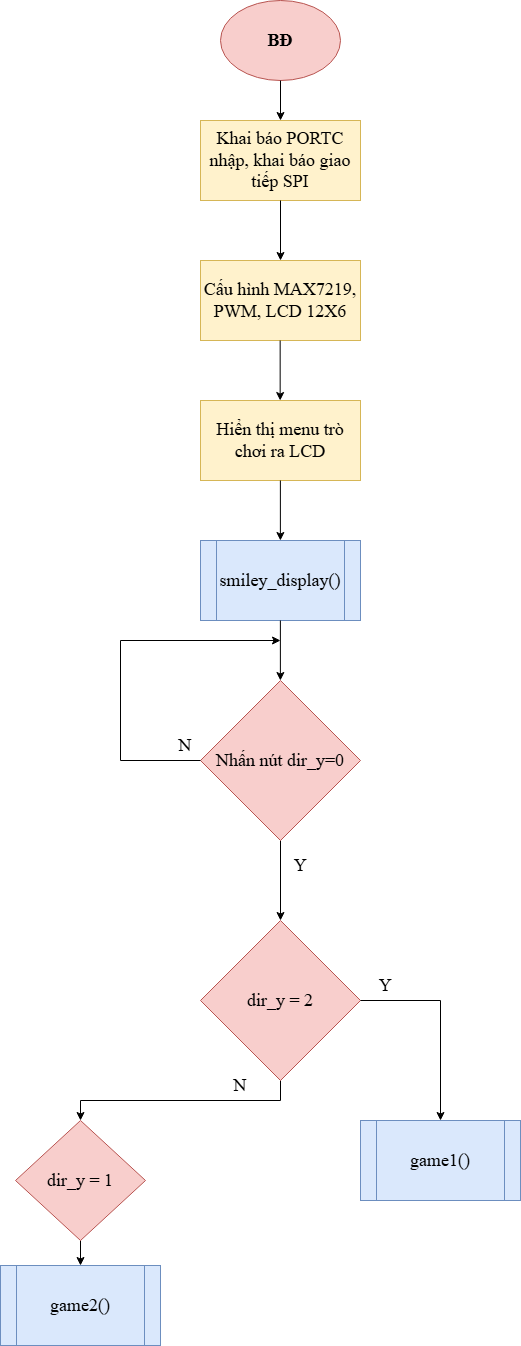
\includegraphics[width=.3\textwidth]{img/main_struct.png}
    \caption{Lưu đồ giải thuật tổng quát}
\end{figure}
\subsection{Lưu đồ giải thuật chi tiết và giải thích:}
\subsubsection{Giải thuật trò chơi snake game}
Lưu đồ chi tiết cho game “rắn săn mồi” bắt đầu bằng bước khởi tạo các biến của trò chơi: chiều dài ban đầu của rắn, vị trí các đốt, hướng di chuyển mặc định, vị trí thức ăn đầu tiên và tốc độ. Tiếp đó, chương trình xóa màn hình, vẽ rắn và thức ăn lên bộ đệm ma trận, hiển thị điểm số lên LCD rồi đi vào vòng lặp chính của game.

Trong mỗi vòng lặp, bước đầu tiên là đọc các nút điều hướng. Nếu phát hiện có phím được nhấn và phím đó không làm rắn quay ngược lại 180 độ so với hướng hiện tại, chương trình cập nhật hướng di chuyển mới. Sau đó, vị trí đầu rắn mới được tính bằng cách cộng thêm vector hướng vào tọa độ đầu cũ. Các đốt phía sau được dịch chuyển lần lượt để “theo” đầu rắn: mỗi đốt nhận vị trí của đốt ngay phía trước trong mảng.

Sau khi cập nhật thân rắn, chương trình lần lượt kiểm tra các điều kiện va chạm. Nếu đầu rắn đi ra ngoài phạm vi ma trận hoặc trùng với bất kỳ đốt nào của chính nó, trò chơi kết thúc. Nếu đầu rắn trùng với vị trí thức ăn, điểm số được tăng lên, độ dài rắn được kéo dài thêm một đốt và hệ thống tạo một vị trí thức ăn mới sao cho không trùng với thân rắn hiện có. Ngược lại, nếu không ăn mồi, độ dài rắn giữ nguyên.

Khi các kiểm tra va chạm hoàn tất, chương trình xây dựng lại bộ đệm hiển thị: xóa toàn bộ nội dung cũ, vẽ từng đốt rắn và ô thức ăn vào đúng vị trí. Bộ đệm này sau đó được gửi sang MAX7219 để hiển thị lên ma trận LED. Cùng lúc, nếu có sự kiện kết thúc trò chơi, chương trình kích hoạt buzzer phát âm thanh tương ứng. Vòng lặp tiếp tục sau một khoảng trễ xác định bởi tham số tốc độ, cho đến khi xảy ra điều kiện “Game Over”, khi đó lưu đồ chuyển sang khối xử lý kết thúc game giống như phần mô tả trong lưu đồ tổng quát.
\begin{figure}[h!]
    \centering
    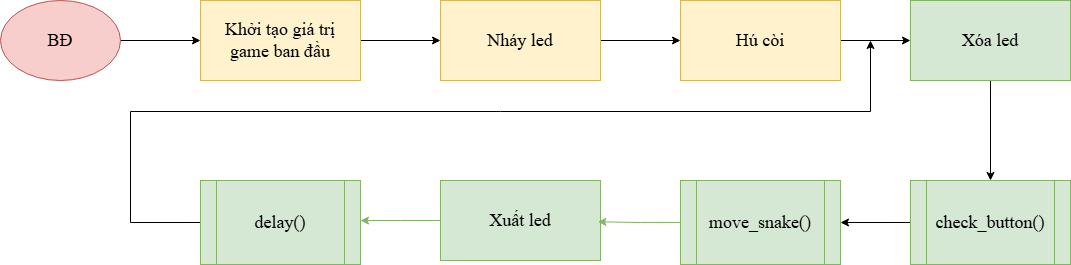
\includegraphics[width=.7\textwidth]{img/6.png}
    \caption{Lưu đồ giải thuật game snake}
\end{figure}
\subsubsection{Giải thuật trò chơi “pickle ball”}
Lưu đồ chi tiết của game “pickle ball” bắt đầu bằng việc khởi tạo vị trí ban đầu của thanh trượt và quả bóng, cùng hai biến thể hiện hướng di chuyển của bóng theo hai trục. Thanh trượt được đặt ở hàng dưới cùng của ma trận, bóng được đặt ở vị trí bất kỳ trong vùng chơi, hướng bóng được chọn sao cho bóng bay về phía thanh trượt. Điểm số được đặt về 0, tốc độ được chọn phù hợp.

Trong vòng lặp chính, chương trình trước tiên đọc các nút điều hướng sang trái hoặc sang phải để cập nhật vị trí thanh trượt, bảo đảm thanh trượt luôn nằm gọn trong phạm vi ma trận. Sau đó, vị trí mới của bóng được tính bằng cách cộng hướng theo trục ngang và dọc vào tọa độ hiện tại. Nếu bóng chạm vào tường trái hoặc phải, hướng ngang của bóng được đảo ngược; nếu bóng chạm vào mép trên, hướng dọc được đảo ngược, tạo cảm giác bóng nảy.

Khi bóng tiến gần hàng dưới cùng, chương trình kiểm tra xem cột của bóng có nằm trong vùng phủ của thanh trượt hay không. Nếu có, bóng được coi là đã đập trúng thanh trượt, hướng dọc của bóng được đảo chiều. Nếu bóng đi xuống dưới mà không gặp thanh trượt, game kết thúc, chương trình hiển thị thông báo thua cuộc và đồng thời phát âm thanh báo hiệu khác biệt.

Trong mỗi chu kỳ, sau khi tính toán xong các vị trí, phần mềm xóa bộ đệm hiển thị, vẽ lại thanh trượt và bóng ở vị trí mới, rồi gửi toàn bộ dữ liệu sang IC điều khiển ma trận LED. Tương tự trò rắn, vòng lặp chỉ dừng lại khi xảy ra điều kiện kết thúc, sau đó lưu đồ chuyển sang lại hay quay lại menu chính (nếu nhấn nút reset).

Với cách tổ chức như trên, phần mềm của BKONSOLE vừa đáp ứng được các yêu cầu chức năng và kỹ thuật đã đặt ra, vừa bảo đảm tính mạch lạc, dễ hiểu và thuận lợi cho việc mở rộng thêm các trò chơi hoặc nâng cấp phần cứng trong tương lai.
\begin{figure}[h!]
    \centering
    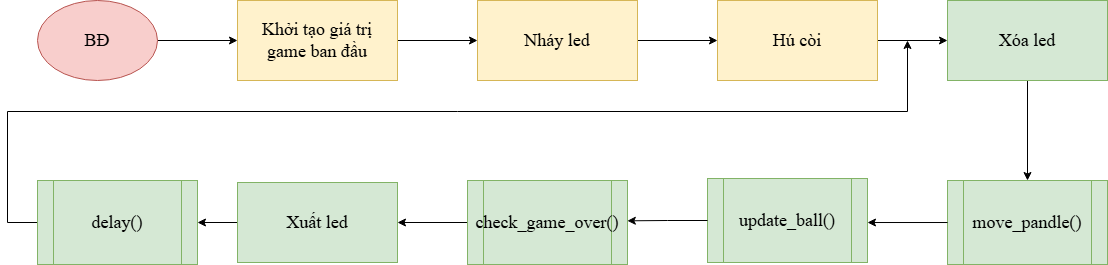
\includegraphics[width=.7\textwidth]{img/7.png}
    \caption{Lưu đồ giải thuật game pickel ball}
\end{figure}